\documentclass[12pt]{article}

\usepackage[margin=1in]{geometry} 
\usepackage{amsmath,amsthm,amssymb}

% новая команда \RNumb для вывода римских цифр
\newcommand{\RNumb}[1]{\uppercase\expandafter{\romannumeral #1\relax}}

%%% Работа с русским языком
\usepackage{cmap}					% поиск в PDF
\usepackage{mathtext} 				% русские буквы в фомулах
\usepackage[T2A]{fontenc}			% кодировка
\usepackage[utf8]{inputenc}			% кодировка исходного текста
\usepackage[english,russian]{babel}	% локализация и переносы
\usepackage{physics} 
 

%%% Работа с картинками
\usepackage{graphicx}  % Для вставки рисунков
\graphicspath{{images/}{images2/}}  % папки с картинками
\setlength\fboxsep{3pt} % Отступ рамки \fbox{} от рисунка
\setlength\fboxrule{1pt} % Толщина линий рамки \fbox{}
\usepackage{wrapfig} % Обтекание рисунков и таблиц текстом
\DeclareGraphicsExtensions{.pdf,.png,.jpg}

%%% Работа с таблицами
\usepackage{array,tabularx,tabulary,booktabs} % Дополнительная работа с таблицами
\usepackage{longtable}  % Длинные таблицы
\usepackage{multirow} % Слияние строк в таблице
\usepackage{rotating}

\usepackage{hyperref}

\usepackage{listings} %For code in appendix
\lstset
{ %Formatting for code in appendix
    language=Python,
    basicstyle=\footnotesize,
    numbers=left,
    stepnumber=1,
    showstringspaces=false,
    tabsize=1,
    breaklines=true,
    breakatwhitespace=false,
}






\begin{document}
%\linenumbers

\begin{center}
    {\bf\LARGE Автоматизированный измерительный стенд} \\
    \vspace{3mm}
    {\sc  Андрей Козий} \\
    \vspace{3mm}
    \today
\end{center}

\vspace{3mm}

%\tableofcontents

%\newpage

\section{Обзор стенда}
Автоматизированный Измерительный Стенд (АИС) предназначен для измерения параметров Детектора Одиночных Фотонов (ДОФ), с последующей программной обработкой полученных данных и формирования отчетов по эксплуатационным характеристикам устройств. 

Принципиальная схема стенда представлена на рисунке \ref{fig:stand_scheme}. Черные стрелки обозначают контакт двух устройств с использованием проводов, желтые -- оптоволокна.  

\begin{figure}[h]\centering
	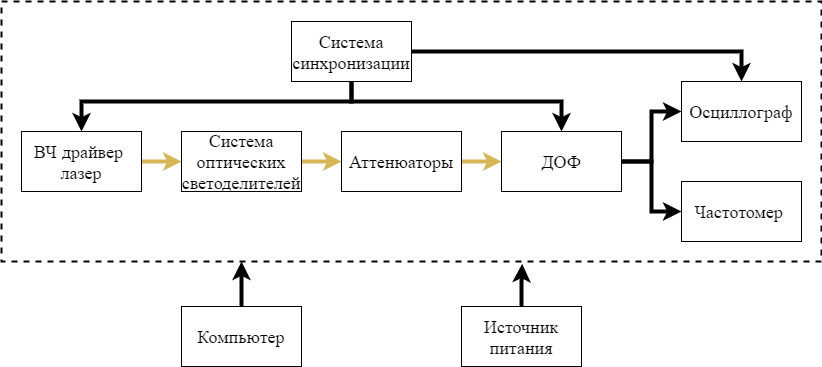
\includegraphics[width=1\textwidth]{stand_scheme}
   \caption{Принципиальная схема автоматизированного измерительного стенда.}
   \label{fig:stand_scheme}
\end{figure}

На рисунке \ref{fig:full_stand} представлена фотография измерительного стенда.

\begin{figure}[h]\centering
	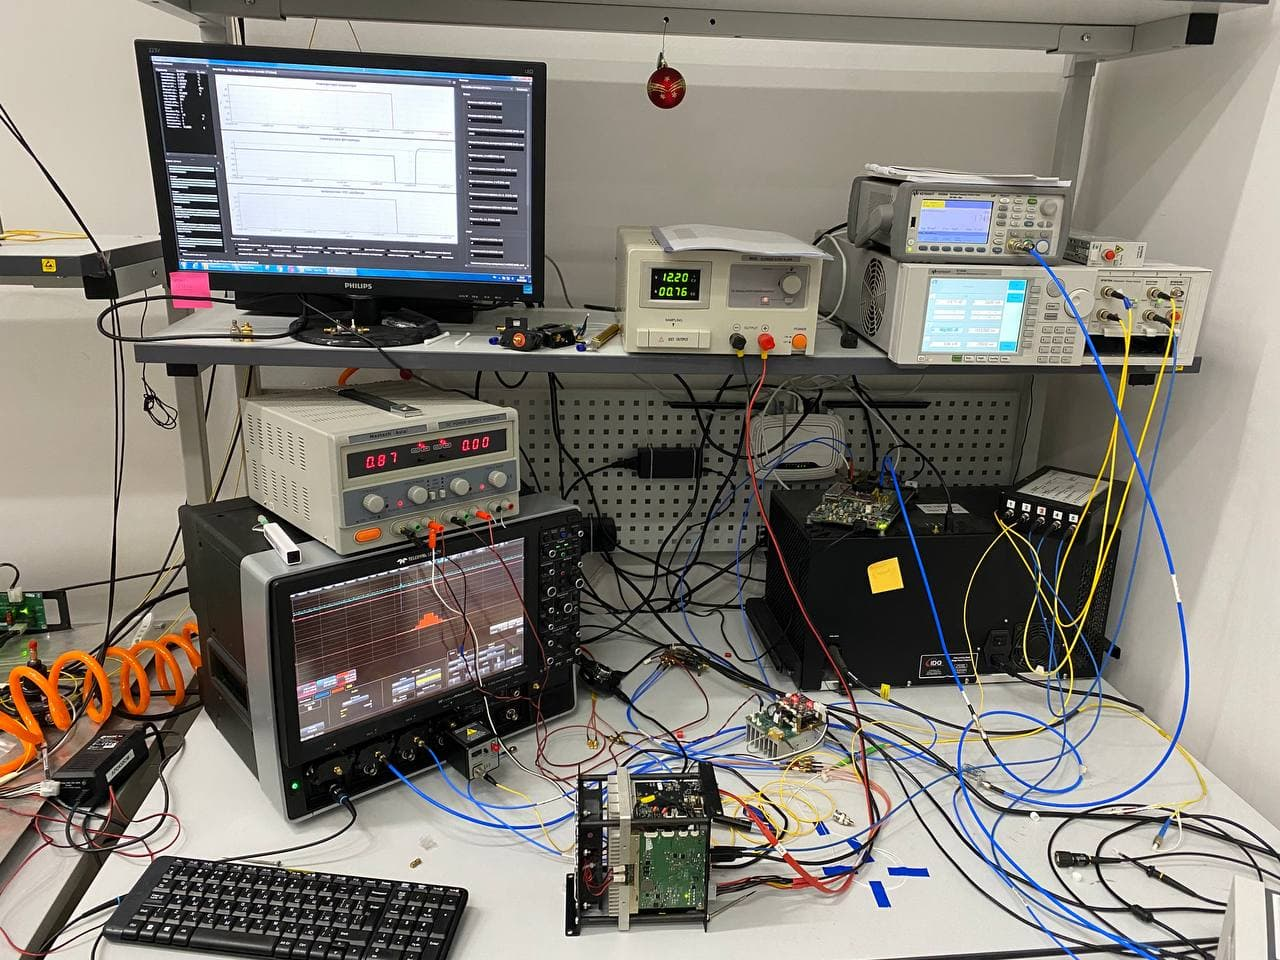
\includegraphics[width=1\textwidth]{full_stand}
   \caption{Фотография измерительного стенда.}
   \label{fig:full_stand}
\end{figure}

На рисунке \ref{fig:stand_pics} представлены фотографии отдельных узлов измерительного стенда. 

\begin{figure}[h]\centering
	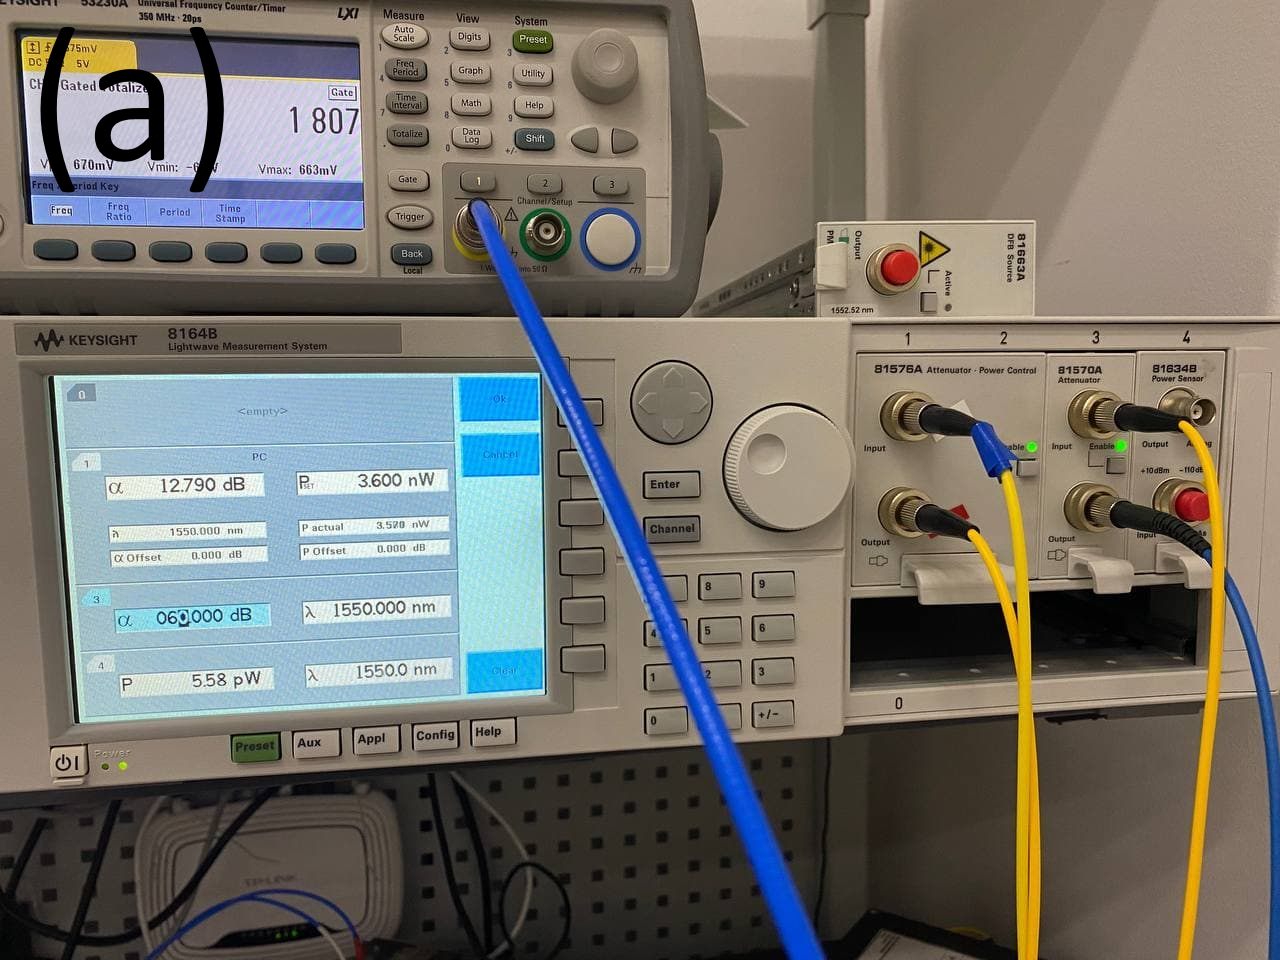
\includegraphics[width=0.3\textwidth]{attenuators}
    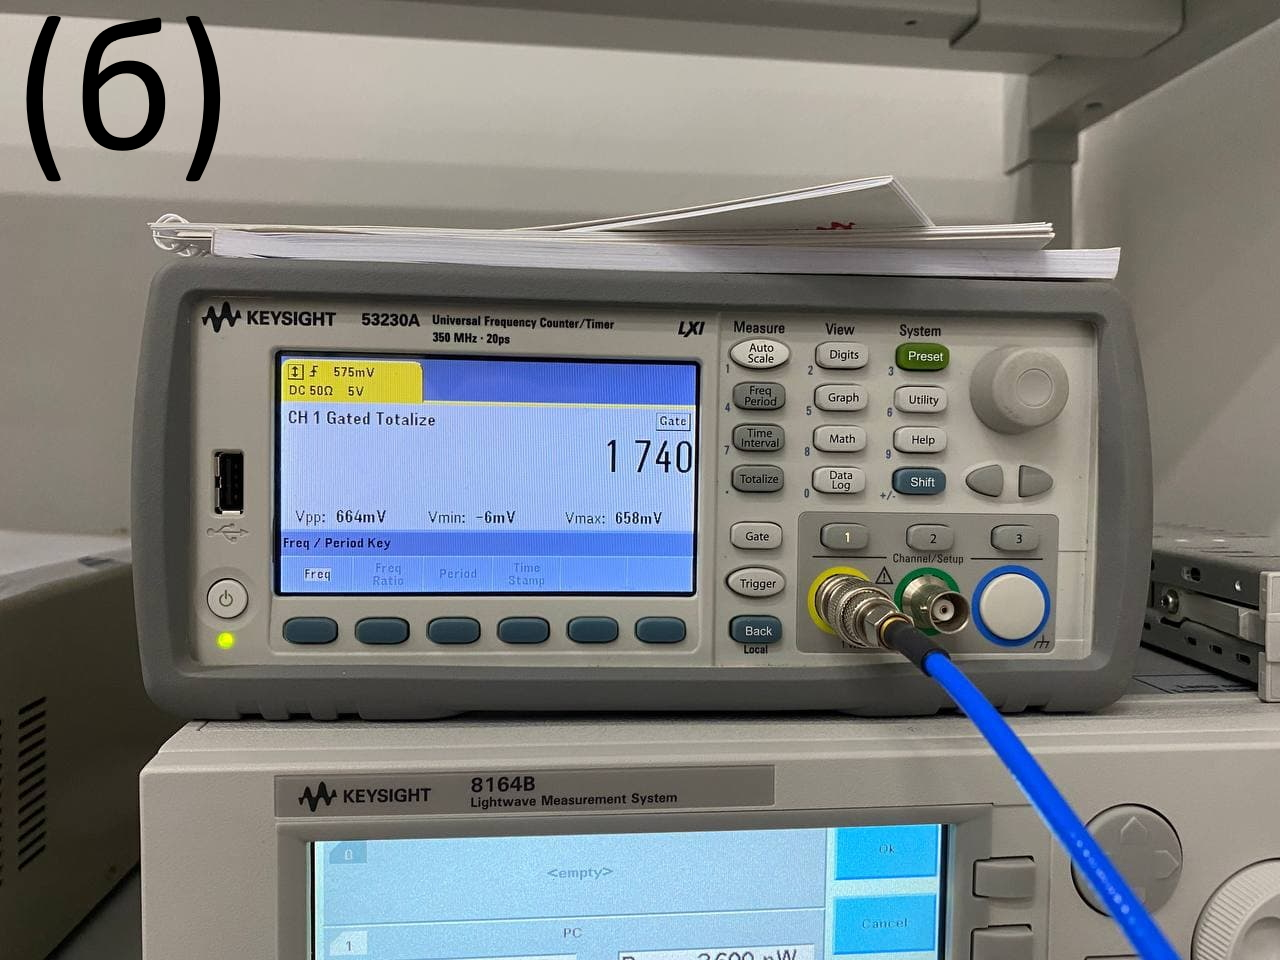
\includegraphics[width=0.3\textwidth]{frequency_meter}
    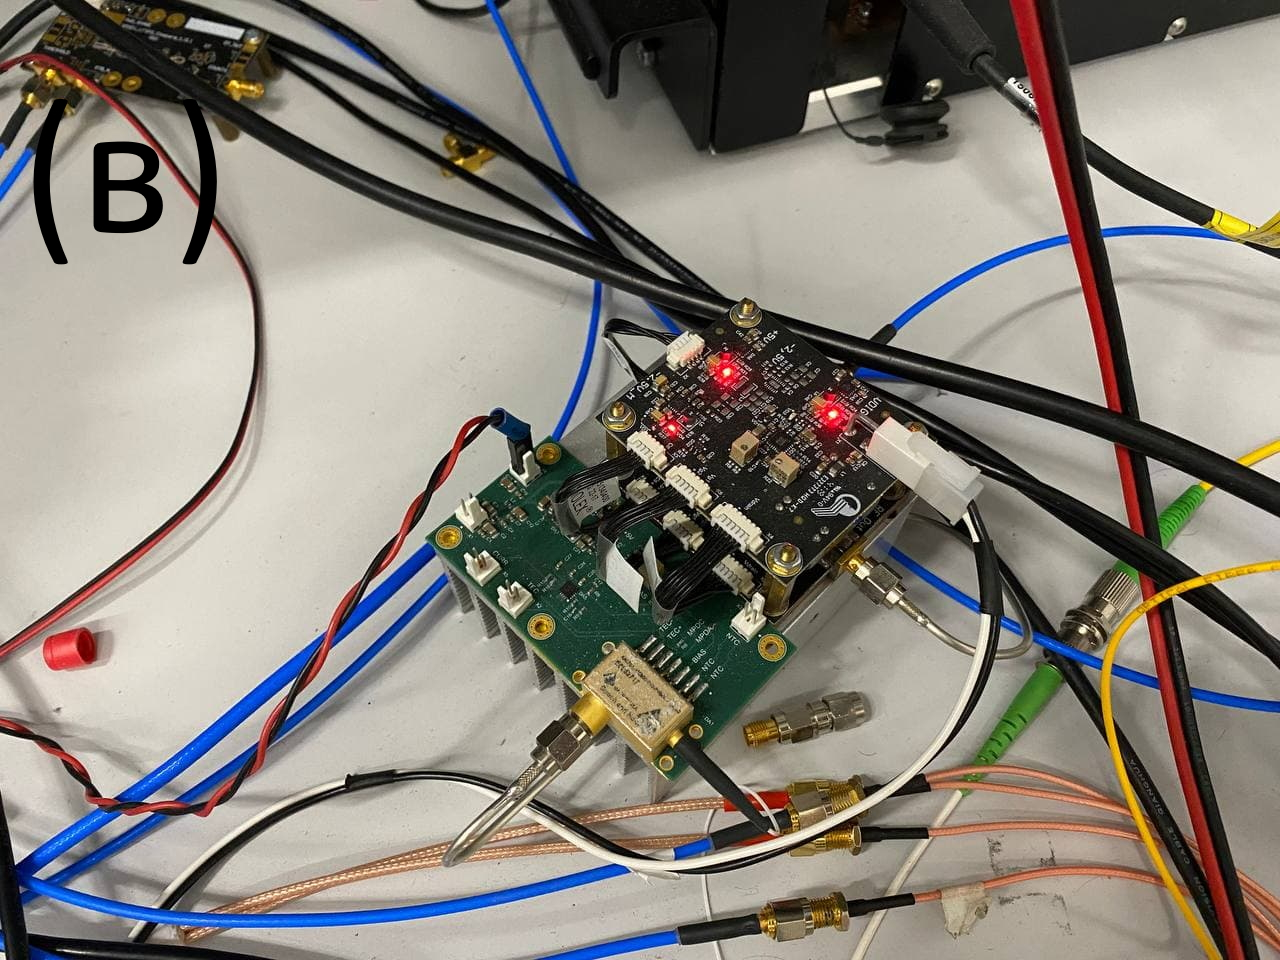
\includegraphics[width=0.3\textwidth]{laser_driver}
    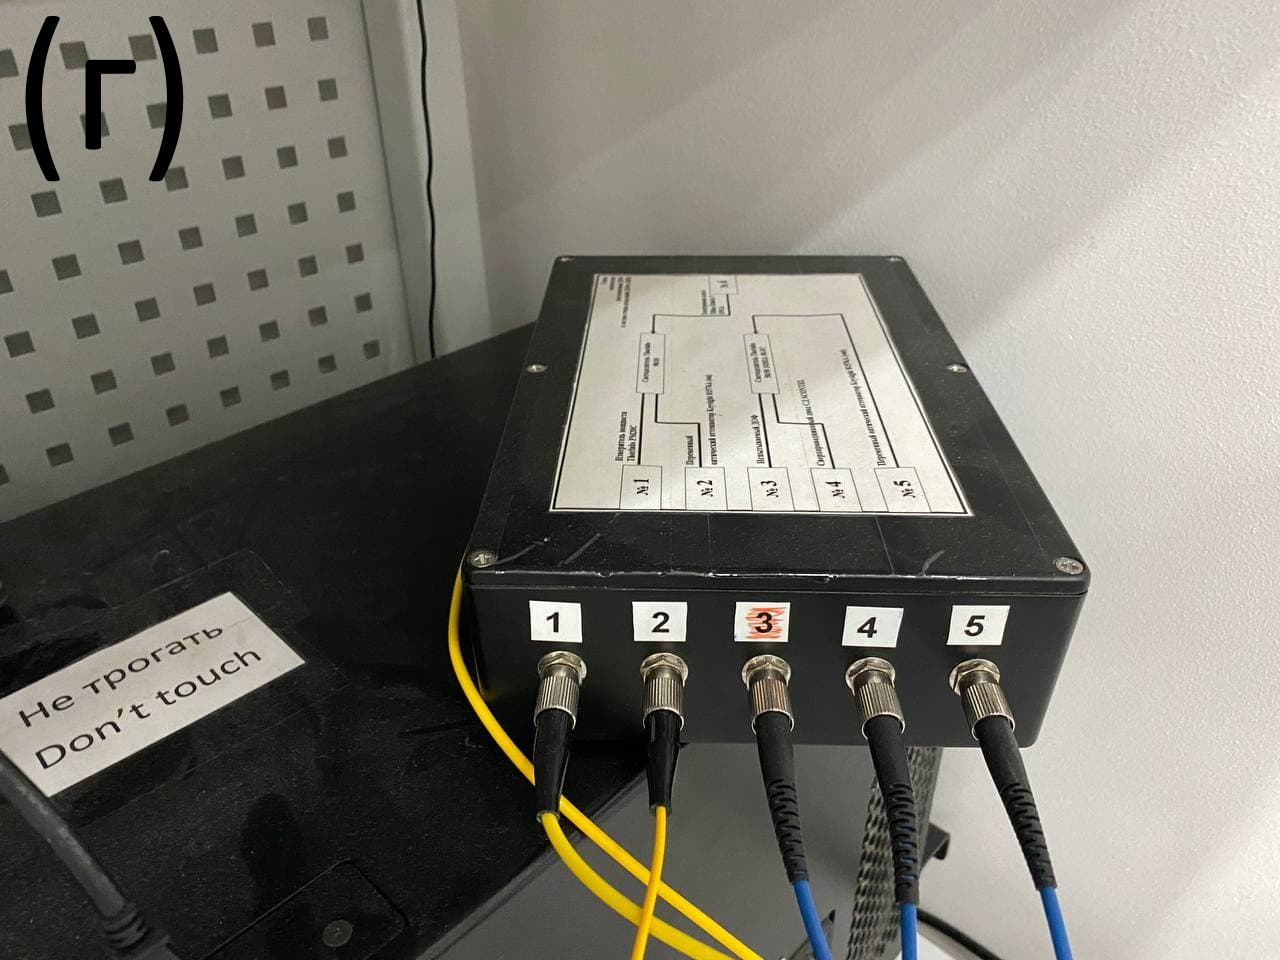
\includegraphics[width=0.3\textwidth]{optical_scheme}
    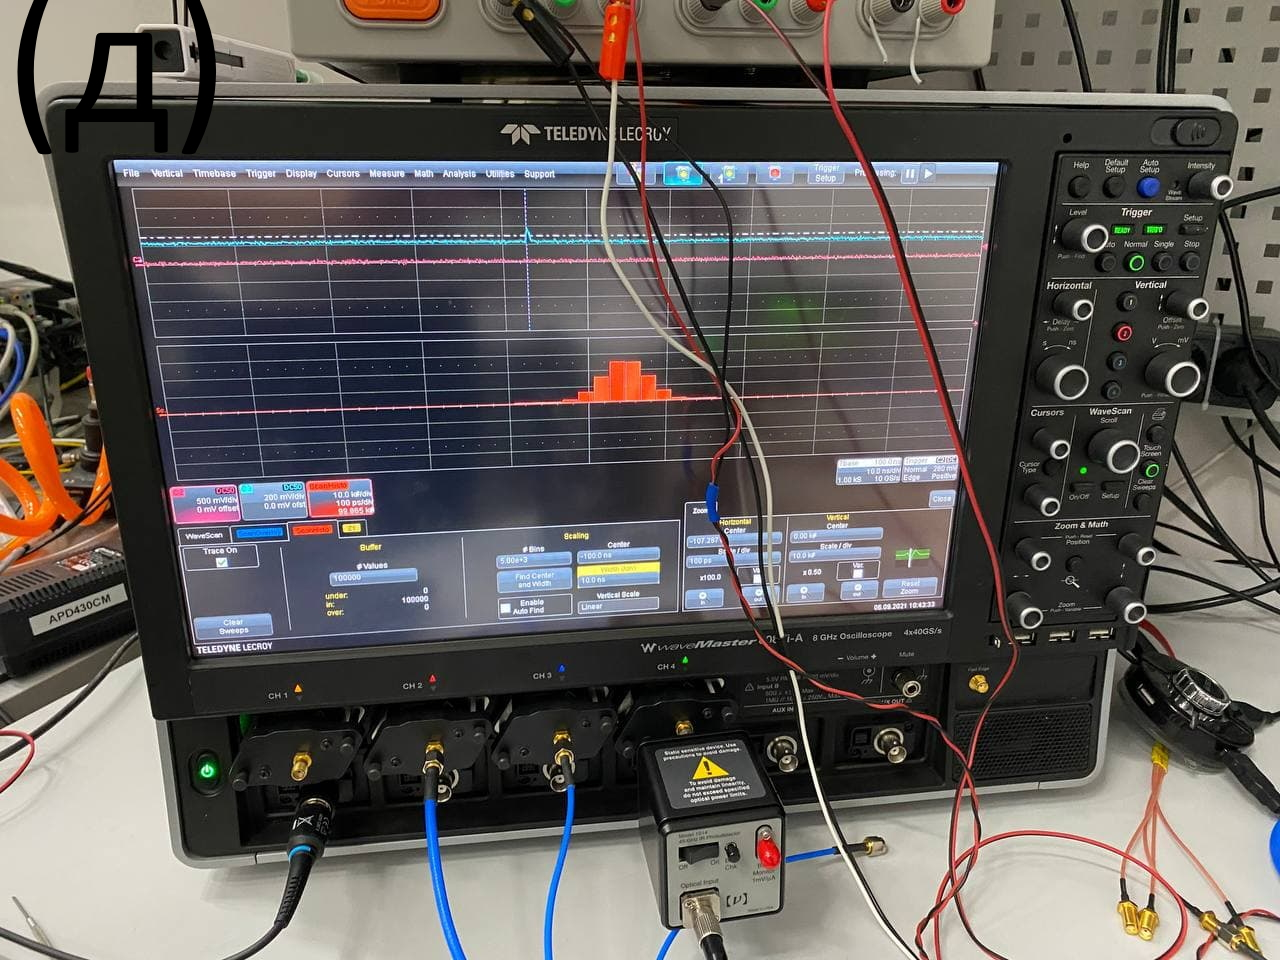
\includegraphics[width=0.3\textwidth]{oscill}
    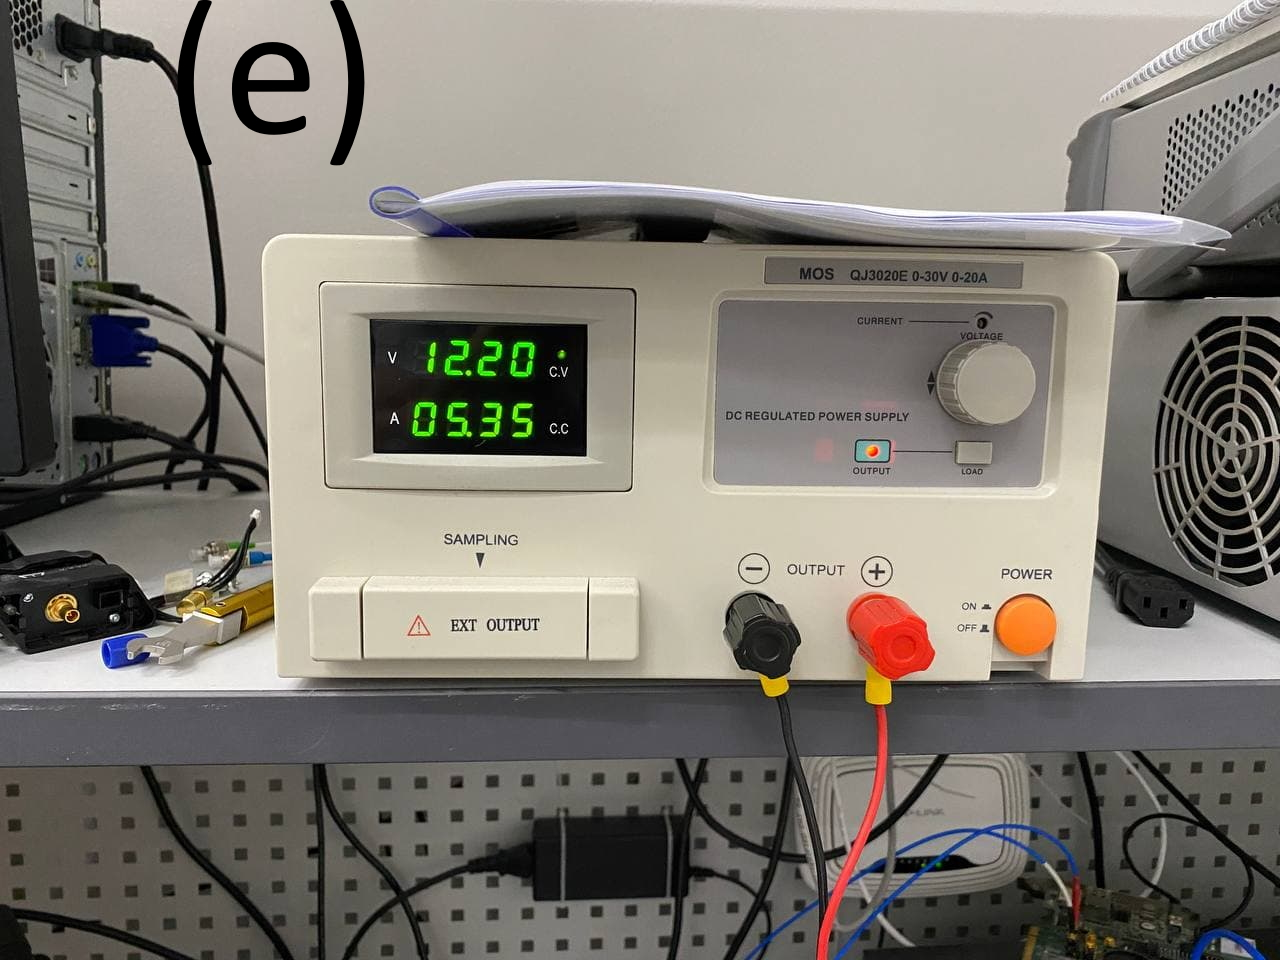
\includegraphics[width=0.3\textwidth]{power_supply}
    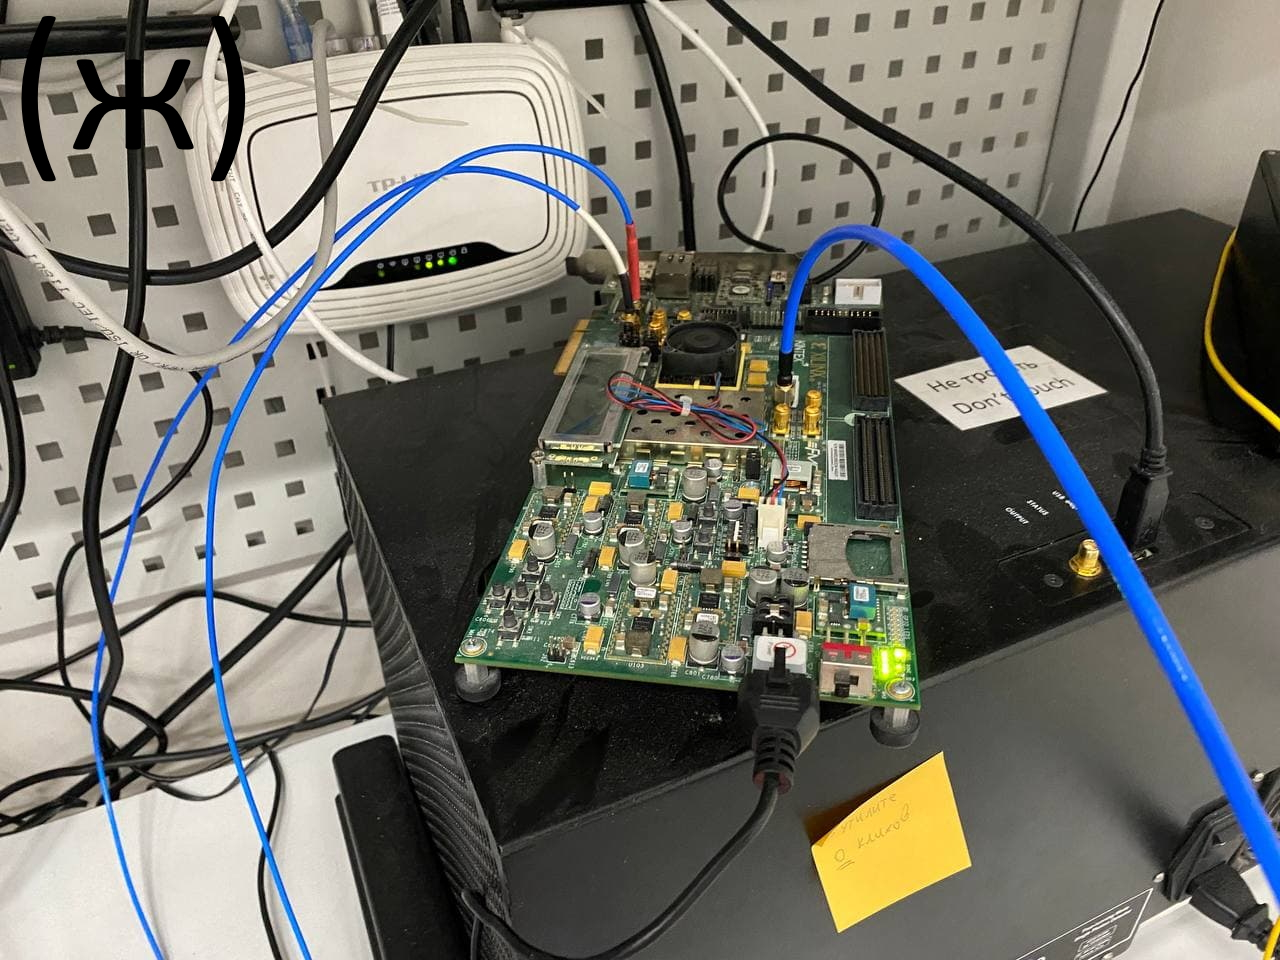
\includegraphics[width=0.3\textwidth]{synchronization}
    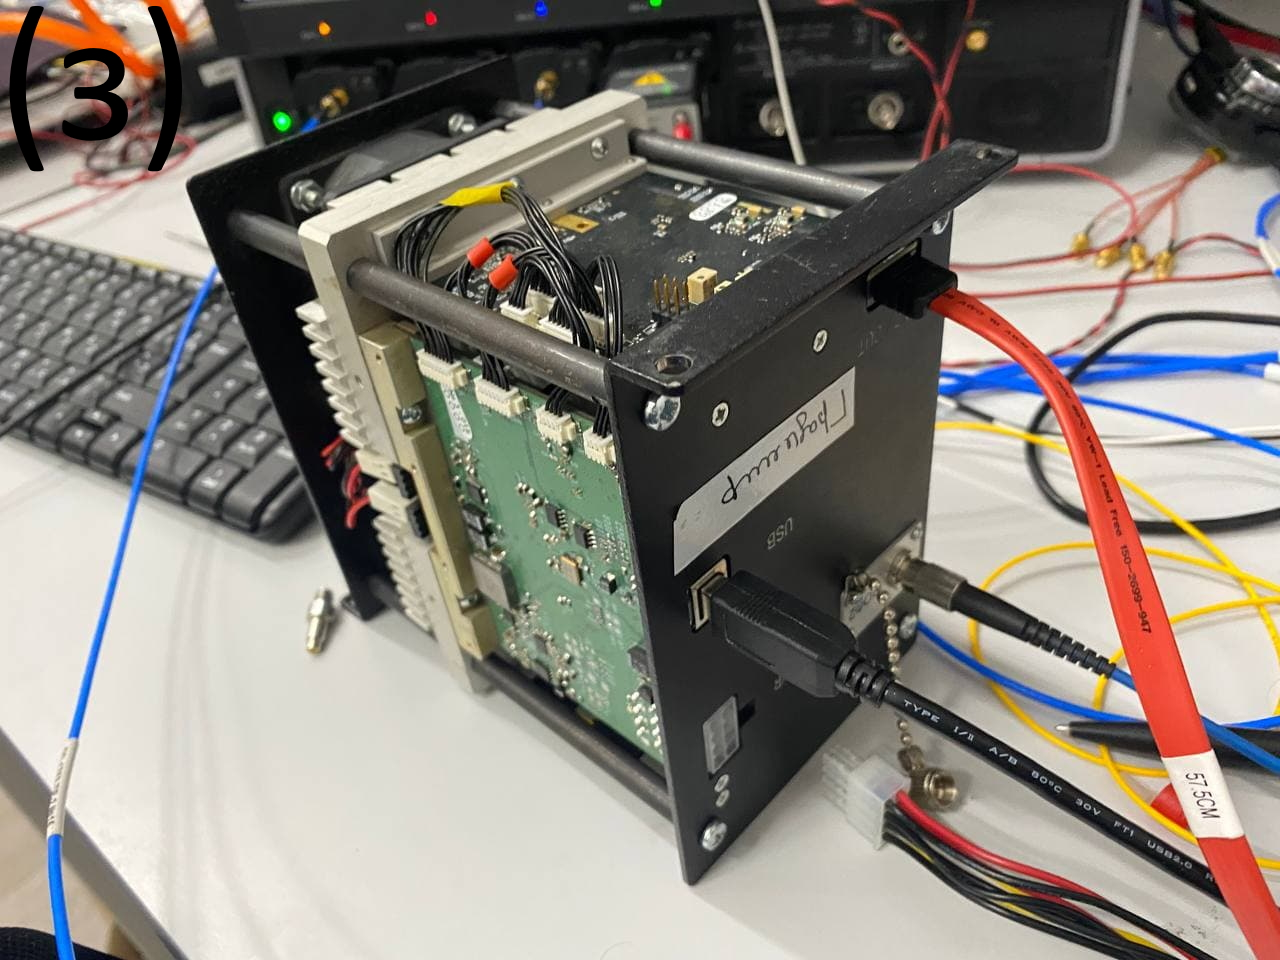
\includegraphics[width=0.3\textwidth]{spd}
    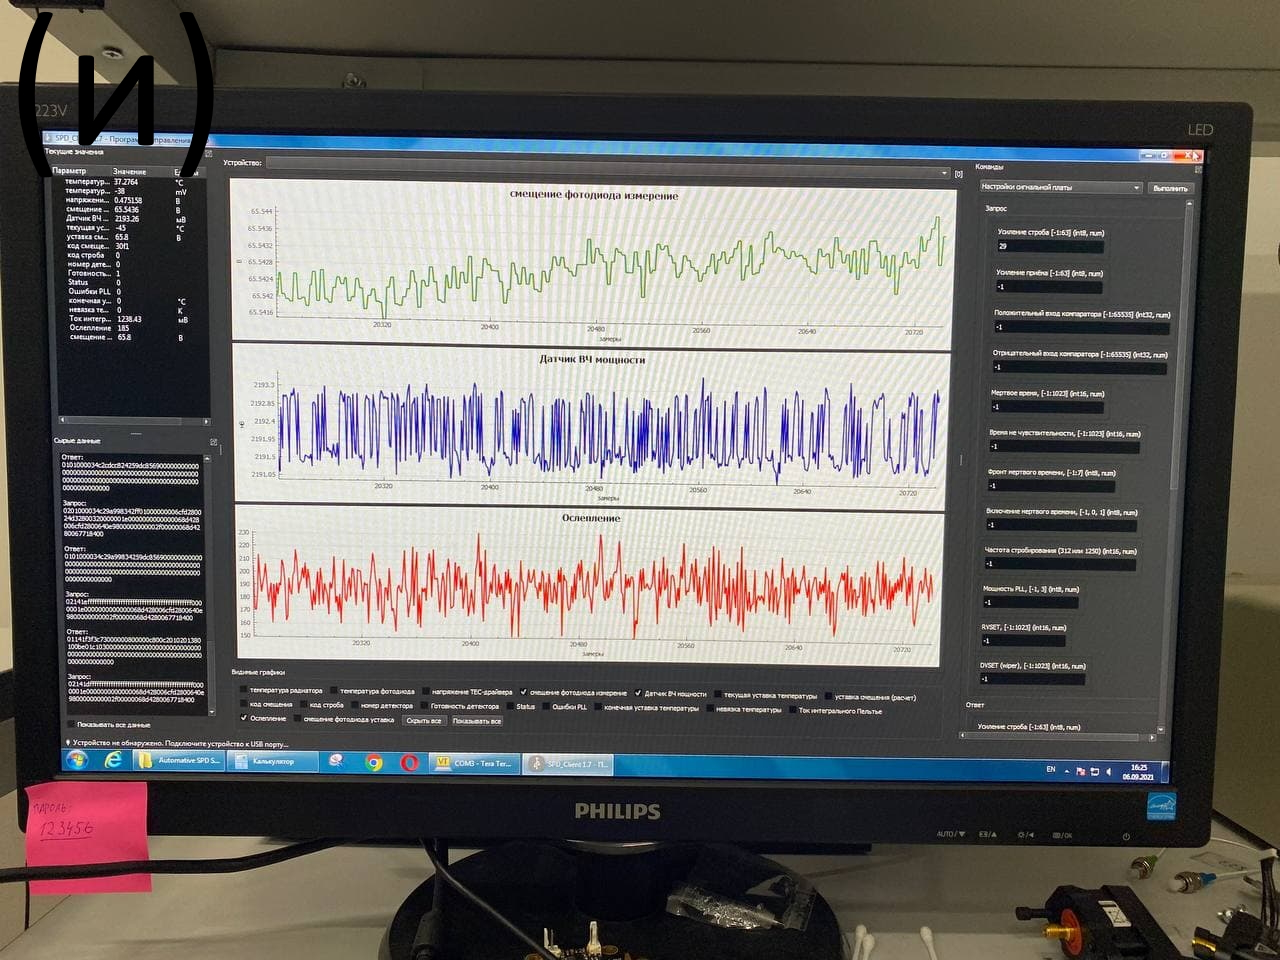
\includegraphics[width=0.3\textwidth]{comp}
   \caption{Фотографии отдельных узлов измерительного стенда. а) блок с аттенюаторами; б) частотомер; в) ВЧ драйвер лазера; г) система оптических светоделителей; д) осциллограф; е) источник питания; ж) схема синхронизации; з) детектор одиночных фотонов: и) компьютер. }
   \label{fig:stand_pics}
\end{figure}


Система синхронизации позволяет генерировать лазерные импульсы и стробы в ДОФ в одной сетке с частотой 312.5 МГц. Синхро-импульсы передаются на три блока -- ВЧ драйвер лазера, ДОФ и осциллограф. Сигнал, приходящий на ВЧ драйвер и на осциллограф имеет одинаковую форму, но отличается только по амплитуде. 

ВЧ драйвер лазера управляет формой лазерного импульса и периодом его следования в частотной сетке, определенной системой синхронизации. Используемая частота следования лазерных импульсов: 10 кГц, 100 кГц, 156.25 МГц, 312.5 МГц (другие на практике не используются).

Лазерные импульсы передаются в систему оптических светоделителей, где одно из выходных направлений используется для последующей передачи оптического излучения на аттенюаторы. 

Для ослабления лазерного излучения используется система из двух последовательно соединенных аттенюаторов. Первый аттенюатор обладает встроенным измерителем мощности на выходе. Это позволяет поддерживать и точно контролировать мощность выходного оптического излучения. Второй аттенюатор настроен на постоянное поглощение в 60 dB. 

После системы аттенюаторов сильно ослабленное световое излучение (со средним числом фотонов на импльс 0.1 -- 1, в зависимости от типа проводимых измерений) передается на детектор одиночных фотонов, где и происходит регистрация. 

Электрический сигнал с ДОФ передается на частотомер и осциллограф. По частотомеру определяется скорость счета и благодаря простым математическим преобразованиям вероятность детектирования фотона $PDE$. На осциллографе, используя сигнал с ДОФ как опорный, и регистрируя импульсы системы синхронизации, можно получать гистограммы распределения послеимпульсов и временного разрешения. 

Источник питания и компьютер, которые вынесены за пунктирный прямоугольник, подключены к каждому элементу данной системы, исключая систему оптических светоделителей. Компьютер используется для управления каждым блоком данной системы, и для обработки приходящих с них данных. 


Далее будет представлено 2 раздела, описывающих работу автоматизированного стенда. В разделе "Алгоритм и настройка измерений" будет подробно описан алгоритм снятия параметров и управления используемых узлов, а также  структура файлов настройки параметров измерения стенда. В разделе "Описание программы обработки" будет описана  структура скриптов для работы GUI и формирования отчетов.  


\section{Алгоритм и настройка измерений}
Настройка измерений задается с помощью трех файлов: \\ \verb|"Equipment.txt"| -- файл с основными параметрами, в котором определяются подключаемые блоки;  \verb|"SPDConfig_strobe.txt"| -- файл с параметрами измерений для детектора стробированного типа; \verb|"SPDConfig_freerun.txt"| -- файл с параметрами измерений для детектора типа фриран. 

\subsection{Файл Equipment}

В данном файле устанавливается информация об адресах подключаемого оборудования в локальной сети. Сам детектор \verb|DevBAlias|  подключается через порт  \verb|COM3|, частотомер \verb|FreqCAlias| имеет адрес \verb|KeySight_53230A|, блок с аттенюаторами \verb|8164BIPAddress| имеет адрес \verb|192.168.1.101|, осциллограф \verb|ScopeAlias| имеет адрес \verb|LeCroy|. 

\begin{lstlisting}
   [Equipment]
   DevBAlias = COM3
   FreqCAlias = KeySight_53230A
   8164BIPAddress = 192.168.1.101
   ScopeAlias = LeCroy
\end{lstlisting}


\subsection{Файл SPDConfig-strobe}


\qquad 0. Тест отсутствия импульса. Проводится как первый этап тестирования сразу после того, как детектор вышел на режим и пользователем была нажата кнопка на проведение первого тестирования. \verb|HV_Bias| задает напряжение смещения на детекторе. Код строба выставляется в 0.  \verb|FreqC_GateTime| определяет время проведения данного тестирования в секундах.

\begin{lstlisting}
   [Test00_NoPulses]
   HV_Bias = 40
   FreqC_GateTime = 1
\end{lstlisting}

1. Тест наличия срабатываний детектора. Проводится автоматически после нулевого этапа. Код строба устанавливается 0. Начиная с напряжения \verb|HV_Bias_Quick_Start| и до напряжения \verb|HV_Bias_Quick_Stop|, изменяется напряжение на детекторе с шагом \verb|HV_Bias_Quick_Step|. Каждый шаг проводятся измерения в течение времени \\ \verb|FreqC_Quick_GateTime| в секундах. Когда грубым шагом удалось получить значения темнового счета $DCR$ больше величины \verb|PulsesCount_min|, шаг заменяется на более малый \verb|HV_Bias_Precise_Step|, а время измерения заменяется на \verb|FreqC_Precise_GateTime|. Таким образом, напряжение будет изменяться на малый шаг как в сторону уменьшения, так и увеличения, пока не будет получено значение темнового счета  \verb|PulsesCount_max|. 

\begin{lstlisting}
   [Test01_HV_bias]
   FS = 100
   TS = 2
   HV_Bias_Quick_Start = 50
   HV_Bias_Quick_Stop = 80
   HV_Bias_Quick_Step = 0,5
   FreqC_Quick_GateTime = 0,5
   HV_Bias_Precise_Step = 0,05
   FreqC_Precise_GateTime = 0,5
   PulsesCount_max = 300
   PulsesCount_min = 200
\end{lstlisting}

2. Тест настройки фазы. Проводится автоматически после первого этапа. Проводится только для стробированного детектора. Устанавливается частота следования лазерных импульсов \verb|FS| в кГц, и команда для формирования нужной ширины лазерного импульса \verb|TS|. Длина волны излучения лазера, используемая во внутренних вычислениях \verb|Laser_WaveLength|. Параметр \verb|P_units = 1| показывает, что далее устанавливается мощность в размерности Вт. На выходе первого аттенюатора контролируется мощность \verb|P_set|. Установленное затухание на втором аттенюаторе \verb|Att|. Параметры выбираются таким образом, чтобы средняя энергия на импульс равнялась одному фотону. Начальная фаза синхронизации между лазерным импульсом и стробами детектора устанавливается равной \verb|Phase_Quick_Start|. После чего алгоритм начинает смещать фазу на величину \verb|Phase_Quick_Step|, вплоть до значения \verb|Phase_Quick_Stop|. На каждой фазе измерение скорости счета выполняется в течение \verb|FreqC_Quick_Gate|. После того, как указанный диапазон фазы был пройден грубым шагом, устанавливается то значение фазы, при котором была получена максимальная скорость счета. Затем, с шагом \verb|Phase_Step_Precise| происходит смещение как в сторону меньшей, так и в сторону большей фазы, на число шагов, равное 10(5). В каждой точке скорость счета определяется за время \verb|FreqC_Precise_Gate|. 


\begin{lstlisting}
   [Test02_Strobe_Phase]
   FS = 100
   TS = 2
   Laser_WaveLength = 1550
   P_units = 1
   P_set = 3,6E-9
   Att = 50
   Phase_Quick_Start = 0
   Phase_Quick_Stop = 300
   Phase_Quick_Step = 10
   FreqC_Quick_Gate = 0,2
   Phase_Step_Precise = 1
   FreqC_Precise_Gate = 1
\end{lstlisting}


3. Измерение сетки. После завершения тестов, можно перейти на следующее окно, в котором необходимо задать параметры последующих измерений. В числе данных параметров следующие: начальная и конечная температура, шаг измерения. В случае, если исследуется стробируемый детектор, то можно выставить начальный и конечный код строба, шаг измерения. Для запуска измерений необходимо однократно нажать на  соответствующую кнопку. После этого устанавливается заданная стартовая температура и начинаются измерения. Первым этапом в непосредственных измерениях является измерение сетки. Параметр \verb|HV_Grid_Start| устанавливает начальное значение напряжения смещения, параметр \verb|HV_Grid_Stop| устанавливает максимальное напряжение смещения, выше которого напряжение устанавливаться не будет. Если напряжение смещения преодолело максимально доступное, и при этом скорость темнового счета не стала больше параметра \verb|HV_Grid_Pulse_Count_max|, то строка с данным кодом строба в файле \verb|"Grid_HV_bias.csv"| заполняется величинами \verb|NULL|. Начальный шаг по напряжению смещения устанавливается \verb|HV_Grid_Initial_Step|, каждое измерение проводится \verb|HV_Grid_FreqC_Num_Of_Meas| раз, каждое в течение \verb|HV_Grid_FreqC_Gate_Time|. Как только грубым шагом удалось дойти до такого режима работы детектора, при котором темновой счет больше \verb|HV_Grid_Pulse_Count_min|, включается режим с точным шагом. Данную точку напряжения назовем точкой разветвления. Сначала осуществляется поиск напряжения, при котором значение темнового счета максимально приближено к \verb|HV_Grid_Pulse_Count_min|. Таким образом, одна ветвь идет в сторону уменьшения напряжения. Новый шаг равен грубому шагу деленному пополам, и напряжение уменьшается на значение нового шага, вплоть до момента, пока скорость счета не станет меньше \verb|HV_Grid_Pulse_Count_min|. После этого значение шага снова уменьшается в два раза. После чего напряжение начинает увеличиваться на величину нового шага, пока не станет больше \verb|HV_Grid_Pulse_Count_min|. Затем шаг снова уменьшается и алгоритм повторяется, пока значение шага не станет равным \verb|HV_Grid_Initial_Step / 32|. Затем, с точки разветвления начинается поиск верхней границы напряжения по аналогичному алгоритму, только теперь приближение скорости счета производится до величины \verb|HV_Grid_Pulse_Count_max|. Таким образом, определяются две точки напряжения -- верхнее и нижнее. Если разница между данными значениями меньше \verb|HV_Grid_Minimum_delta_V|, то считается, что доминирует эффект захвата зарядов (charge persistence), в результате чего такой режим работы детектора не может являться оптимальным, и его измерение, и измерение всех больших кодов строба не имеет смысла. В массив сетки на строки соответствующих кодов строба заносится значение \verb|NULL|, и алгоритм измерения переходит к следующему шагу. В случае, если разница между напряжениями больше величины \verb|HV_Grid_Minimum_delta_V|, то формируется одномерная линейная сетка напряжений для данного кода строба, с числом точек, равное \verb|HV_Grid_HV_bias_Number_Of_Intervals|. Аналогичный алгоритм выполняется для следующего кода строба. Таким образов, для детектора стробированного режима для выбранной температуры, сетка напряжений представляется в виде двумерного массива. Для детектора типа фриран -- в виде одномерного массива. 
 

\begin{lstlisting}
   [Test03_Measurments_Grid]
   HV_Grid_FS = 100
   HV_Grid_TS = 2
   HV_Grid_Start = 50
   HV_Grid_Stop = 80
   HV_Grid_Initial_Step = 1
   HV_Grid_FreqC_Gate_Time = 0,1
   HV_Grid_FreqC_Num_Of_Meas = 10
   HV_Grid_Pulse_Count_min = 30
   HV_Grid_Pulse_Count_max = 2000
   HV_Grid_Minimum_delta_V = 0,4
   HV_Grid_HV_bias_Number_Of_Intervals = 10
\end{lstlisting}

4. Измерение $DCR$. Для каждой точки сетки напряжений и кодов строба выполняется измерение темнового счета -- всего \verb|DCR_FreqC_Num_Of_Meas| измерений, каждое в течение \verb|DCR_FreqC_Gate_Time|. Данный подход необходим для вычисления значения среднеквадратического отклонения. В результате чего создается два файла -- \verb|"DCR.csv"| и \verb|"DCRSigma.csv"|.


\begin{lstlisting}
   [Test04_Measurments_DCR]
   DCR_FS = 100
   DCR_TS = 2
   DCR_FreqC_Gate_Time = 0,1
   DCR_FreqC_Num_Of_Meas = 30
\end{lstlisting}

5. Измерение скорости счета со включенным излучением и временного разрешения. Для каждой точки сетки напряжений и кодов строба выполняется алгоритм настройки фазы, аналогичный описанному в пункте 2 -- тестирование настройки фазы. Только в данных измерениях затухание на втором аттенюаторе устанавливается равным \verb|QE_ATT3|, чтобы среднее число фотонов на импульс равнялось $0.1$.  Измерения в процессе поиска фазы, и непосредственно измерение после настройки фазы, выполняется \verb|QE_FreqC_Num_Of_Meas| раз, по \verb|QE_FreqC_Gate_Time| секунд каждое. Это позволяет определить среднеквадратическое отклонение в скорости счета. В результате чего создается два файла -- \verb|"QE.csv"| и \verb|"QESigma.csv"|.

Далее, после проведения измерения скорости счета, проводится измерение временного разрешения с установленной настройкой фазы, в случае, если индекс точки  в составленной сетке напряжений при заданном коде строба больше или равно \\ \verb|TR_Start_Meas_index|. Это обусловлено тем, что в первых точках сетки $PDE$ достаточно мало, и статистика на гистограмме собирается слишком долго. Для измерения статистики используется осциллограф, на котором предварительно загружается настройка с именем \verb|TR_Scope_Recall_File|. Количество собранных измерений на осциллографе задается величиной \verb|TR_Histo_Size|. Данный алгоритм проводится для каждой точки сетки. 
 
\begin{lstlisting}  
   [Test05_Measurments_QE]
   QE_FreqC_Gate_Time = 0,1
   QE_FreqC_Num_Of_Meas = 30
   QE_ATT3 = 60
   TR_Start_Meas_index = 5
   TR_Scope_Recall_File = spd-jitter-setup--00003.lss
   TR_Histo_Size = 10000
\end{lstlisting}

6. Измерение послеимпульса. Режим работы лазера переключается на частоту следования импульсов \verb|AP_FS| кГц. Затухание на постоянном аттенюаторе устанавливается \verb|AP_ATT3|, чтобы количество фотонов на импульс составляло 1, с целью увеличения скорости сбора статистики. На осциллографе загружается файл настройки \\ \verb|AP_Scope_Recall_File|. Следующий алгоритм выполняется только для двух точек сетки по каждому коду строба -- самой правой и центральной. Для каждой выбранной точки сначала устанавливается фаза, по описанному в пункте 2 алгоритму. При поиске фазы выполняется \verb|AP_FreqC_Num_Of_Meas| измерений по \verb|AP_FreqC_Gate_Time| секунд, в каждой точке фазы. После чего запускается сбор статистики. Остановка происходит по достижению количества собранных срабатываний \verb|AP_Histo_Size|.  


\begin{lstlisting}
   [Test06_Measurments_AP]
   AP_FS = 10
   AP_TS = 2
   AP_ATT3 = 60
   AP_FreqC_Gate_Time = 0,1
   AP_FreqC_Num_Of_Meas = 10
   AP_Scope_Recall_File = spd-ap-setup-100khz--00000.lss
   AP_Histo_Size = 10000
\end{lstlisting}

7. Измерение временного разрешения на высокой частоте. Измерения производятся для каждого кода строба, для точек сетки, чей индекс больше \verb|TR_bif_Start_Meas_index|. Это обусловлено тем, что при меньших индексах малая вероятность детектирования фотона, и статистика собирается в течение нерелевантно большого времени.  Режим работы лазера переключается на частоту \verb|TR_bif_FS|, затухание на втором аттенюаторе \verb|TR_bif_Att3|. В данном случае тоже необходимо выполнить алгоритм настройки фазы, описанный в пункте 2.  Для этого контролируется выходная мощность на первом аттенюаторе  \verb|TR_bif_P_set_phase_tune|. Измерение на каждой точке фазы выполняется \verb|TR_bif_FreqC_Num_Of_Meas| раз, каждое в течение \verb|TR_bif_FreqC_Gate_Time|.  После настройки фазы контролируемая мощность на выходе первого аттенюатора устанавливается \verb|TR_bif_P_set_meas| Вт. На осциллографе загружается настройка с именем \verb|TR_bif_Scope_Recall_File|. Начинается сбор статистики, который заканчивается по достижению количества точек на гистограмме \verb|TR_bif_Histo_Size|. 


\begin{lstlisting}
   [Test07_Measurments_TR_bifurcation]
   TR_bif_FS = 156250
   TR_bif_TS = 2
   TR_bif_Att3 = 60
   TR_bif_P_set_meas = 5,6E-6
   TR_bif_P_set_phase_tune = 500E-9
   TR_bif_FreqC_Gate_Time = 0,1
   TR_bif_FreqC_Num_Of_Meas = 10
   TR_bif_Scope_Recall_File = spd-jitter-setup--00003.lss
   TR_bif_Histo_Size = 100000
   TR_bif_Start_Meas_index = 5
\end{lstlisting}

\subsection{Файл SPDConfig-freerun}

Файл кофигурации для детектора типа фриран имеет ту же самую структуру, что и файл конфигурации для стробированного режима. Он обладает полностью идентичными полями (за исключением шага 7, на котором измеряется временное разрешение на высокой частоте), однако некоторые поля не считываются программой и не участвуют в алгоритме измерений. Для данного типа детектора не нужно использовать алгоритм настройки фазы. 


0. Тест отсутствия импульсов. Выполняется аналогично стробированному режиму.

1. Тест наличия срабатываний детектора. Выполняется аналогично стробированному режиму.

2. Тест настройки фазы. Отключен при тестировании детектора типа фриран. 

3. Измерение сетки. Отличие от стробированного режима заключается в том, что в данном случае отключено изменение кода строба. Для построения всех массивов считает, что измерения проводятся с единственным кодом строба, равным 0. Таким образом,  алгоритм настройки повторяется, как будто для единственного строба. 

4. Измерение $DCR$. Алгоритм проводится аналогично алгоритму для стробированного режима, только для одного кода строба.

5. Измерение скорости счета со включенным излучением и временного разрешения. Алгоритм проведения аналогичен алгоритму для стробированного детектора, только для одного кода строба, и с отключенной функцией подстройки фазы. 

6. Измерение послеимпульса. Проводится аналогично алгоритму для стробированного детектора, только для одного кода строба, и с отключенной функцией подстройки фазы.





\section{Описание программы обработки}

Репозиторий программы обработки доступен по ссылке \href{https://github.com/akoziy98/Automated_Stand}{Автоматизированный Измерительный Стенд}. 

Данный репозиторий обладает следующей структурой: 
\begin{itemize}
   \item Папка \verb|"!SPDStandResults"| содержит папки с измерениями для различных детекторов. Папка с именем детектора содержит папки с датой проведенных измерений. Папка с датой измерения содержит папки \verb|"report"|, папки формата \verb|"T_-*"|, файлы \verb|"ErrorLog.txt"| с логом возникающих при измерениях ошибок, \verb|"SPDConfig_.txt"| являющийся копией файла настройки измерений, \\ \verb|"Grid_Temperature.csv"| с измеряемой сеткой по температуре, и в случае измерения стробируемого детектора файлы \verb|"Grid_Stb_Code.csv"| с измеряемой сеткой по кодам строба, \verb|"gate_voltage.xlsx"| с таблицей перевода кода строба в амплитуду строба для конкретного детектора. 
   
   Папка формата \verb|"T_-*"| содержит папки с кодом строба в шестнадцатиричном формате типа \verb|"0x*"|, файлы \verb|"Grid_HV_bias.csv"| с двумерной сеткой напряжений смещений, в котором каждая строка соответствует конкретному значению кода строба,  \verb|"DCR.csv"| с измеренным темновым счетом в точках сетки, определенных файлом \verb|"Grid_HV_bias.csv"| (далее в точках сетки напряжений); \verb|"DCRSigma.csv"|, \verb|"QE.csv"|, \verb|"QESigma.csv"| со среднеквадратическим отклонением (СКО) для скорости темнового счета, скорости счета при включенном излучении и СКО для скорости счета при включенном излучении соответственно. 
   
   Папка формата \verb|"0x*"| содержит три типа файлов в формате \verb|"AP_*"|, \verb|"TR_*"| и \verb|"TR_Bif_*"|, в названии которого содержится значение напряжения смещения, при котором данное измерение было проведено. В файле  \verb|"AP_*"| представлена статистика с осциллографа для определения послеимпульса, в файле  \verb|"TR_*"| представлена статистика с осциллографа для определения временного разрешения (джиттера) при частоте лазерных импульсов 100 кГц, в файле \verb|"TR_Bif_*"| представлена статистика с осциллографа для определения временного разрешения и забросов срабатываний детектора в строб, в который не приходит лазерное излучение, при частоте лазерных импульсов 156.25 МГц.

   Папка \verb|"report"| содержит папки \verb|"QE"| и \verb|"SNR"|, в которых в качестве оптимальных параметров представлены параметры, полученные при фиксированном $PDE$ с минимальным $DCR$, и при минимальном соотношении сигнал-шум $SNR$ соответственно. Каждая папка содержит графики зависимости различных параметров детектора, а также сформированные отчеты в формате pdf. Отчет, имеющий формат  \verb|"*_CD.pdf"| содержит графики, в которых используется код строба, а отчет формата  \verb|"*_VG.pdf"| содержит графики, в которых используется амплитуда строба. 


   \item Файл \verb|"afterpulse.py"| содержит функцию \verb|Ap_analyze()|, которая определяет мертвое время $DT$ и вероятность послеимпульса  $AP$ по файлам формата \verb|"AP_*"|. 
   
   \item  Файл \verb|"design5.py"| содержит представление GUI дизайна \verb|"design5.ui"|, переведенное в код python. Данная конвертация может быть выполнена командой \verb|$ pyuic5 path/to/design.ui -o output/path/to/design.py| в консоли. Более подробно  это описано в \href{https://tproger.ru/translations/python-gui-pyqt/}{статье про python GUI}. В файле \verb|"design5.py"| определяются такие объекты, как label, line, combobox, slider, button, Widget (окна для отрисовки графиков), задаются координаты их размещения.
   
   \item Файл \verb|"generate_pdf.py"| отвечает за генерацию отчетов в формате pdf. В нем  используется  библиотека fpdf. Кастомизация колонтитулов происходит благодаря переопределению некоторых функций класса \verb|class CustomPDF(FPDF)|. Функция \verb|create_pdf()| размещает на странице pdf уже сгенерированные изображения, в зависимости от типа детектора и используемого критерия. Функция \verb|simple_table()| отвечает за представление таблиц.  
    
   \item Файл \verb|"graphics_generation.py"| отвечает за генерацию различных графиков и их последующее сохранение. Функция \verb|get_sub_slice(qe_sat)| возвращает массивы-срезы различных физических величин, полученные для заданного значения \verb|qe_sat|. Функция \verb|get_slices()| формирует набор массивов-срезов для различных параметров \verb|qe_sat|, благодаря  вызову функции \verb|get_sub_slice(qe_sat)|. Функция  \\ \verb|plot_dcr_qe_fr()| генерирует график $DCR(V_b)$ и $PDE(V_b)$ для ДОФ типа фриран  (freerun).  Функция \verb|plot_dcr()| генерирует график $DCR(V_g)$ для стробированного (gated) ДОФ. Функция \verb|plot_ap_fr()| генерирует график $AP(V_b)$ для ДОФ типа фриран. Функция \verb|plot_ap()| генерирует график $AP(V_g)$ для стробированного ДОФ. Функция \verb|plot_snr_fr()| генерирует график $SNR(V_b)$ для ДОФ типа фриран. Функция \verb|choose_optimum_fr()| осуществляет поиск оптимальных параметров для ДОФ типа фриран по критерию минимального $SNR$ (\verb|criterion = 'SNR'|) и по критерию минимального $DCR$ при заданном $PDE$ (\verb|criterion = 'QE'|). Функция \verb|TR_filtration(cnt)| производит сглаживание джиттера \verb|cnt| с помощью низкочастотного фильтра. Функция \verb|choose_optimum()| осуществляет поиск оптимальных значения для стробированного детектора по критерию минимального $SNR$ и по критерию минимального $DCR$ при заданном $PDE$.  Функция \verb|find_bif(hist)| осуществляет обработку гистограммы из файла \verb|"TR_Bif_*"|, благодаря чему определяется относительное количество забросов кликов детектора в соседний строб. Функция \verb|plot_TR()| генерирует график временного разрешения $TR(t)$ для ДОФ двух типов и для различных критериев оптимальности.  Функция \\ \verb|plot_heatmap_bif()| генерирует тепловую карту для зависимости $BIF(V_g, V_b)$. Функция \verb|plot_heatmap()| генерирует тепловую карту для зависимости $SNR(V_g, V_b)$. Функция \verb|generate_pdf()| вызывает описанные функции генерации графиков, описанные выше, а также вызывает функцию \verb|create_pdf()| из файла \\ \verb|"generate_pdf.py"|. 

   \item Файл \verb|"GUI5.py"| отвечает за взаимодействие в GUI, а именно класс \\ \verb|class ProgramGUI()|, который имеет наследование от классов \\ \verb|QtWidgets.QMainWindow| и  \verb|design5.Ui_MainWindow|. Функция \verb|init_ui()| определяет надписи в лэйблах, и описывает связи событий на различных интерактивных элементах с созданными функциями. Функция \verb|create_report()| вызывает функцию \verb|generate_pdf()| из файла \verb|"graphics_generation.py"|. Функция \\ \verb|directory_view()| реализует просмотр папок с детекторами и их отображение в комбобоксе. Функция \verb|date_view(index)| реализует просмотр папок с датами для выбранного имени детектора. Функция \verb|download_spd()| реализует создание пути к экспериемнтальным данным, на основе выбранных имен в комбобоксах и вызывает функцию \verb|download_files()|. Функция \verb|download_files()| загружает обработанные функцией \verb|SPD()| (из файла \verb|"spd_analyze.py"|) данные по детектору в объект \verb|SPD|. Функция \verb|shift_slider2_newplot()| вызывается при взаимодействии с одним из слайдеров и вызывает перерисовку графических объектов. Функция \verb|shift_slider2()| вызывается при взаимодействии с одним из слайдеров, вычисляет новые массивы-срезы, которые необходимо отобразить. Функция \verb|shift_slider()| работает аналогично функции \verb|shift_slider2()|. Функции \verb|shift_slider()| и \verb|shift_slider2()| работают в паре, для оптимизации количества перерисовываемых объектов. Функция \verb|fill_labels()| заполняет лэйблы в GUI в соответствии с выбранной на графиках точкой. Функция \verb|plot2d_click()| Реализует отрисовку 2-d графиков в соответствии с выбранным \verb|plot_setup|. Функция \verb|plot3d_click()| реализует отрисовку 3-d графиков в соответствии с выбранным \verb|plot_setup|. В функции \verb|main()| инициализируется GUI. 
   
   \item Файл \verb|"module_fwhm.py"|  содержит функции \verb|fwhm(array)| и \verb|fwtm(array)|, которые вычисляют полную ширину на половине высоты и на одной десятой высоты от массива соответственно.
   
   \item Файл \verb|"module_pde.py"| содержит функцию \verb|pde()|, которая вычисляет вероятность детектирования фотона, исходя из собранных статистических данных. 
   
   \item Файл \verb|"spd_analyze.py"| содержит класс для работы с параметрами ДОФ. В инициализации происходит загрузка массива температуры, а по файловой структуре определяется принадлежность устройства к классу фриран или стробированному. Функция \verb|func_exp()| определена для аппроксимации полученных параметров по послеимпульсу из двух точек, на все точки сетки напряжений. Функция \verb|load_freerun()| реализует загрузку всех данных для детектора типа фриран. Вначале для каждой температуры из папки \verb|"0x000"| загружаются гиcтограммы для  послеимпульса, по которым определяются  параметры вероятности послеимпульса $AP$ и мертвое время $DT$. В том же цикле загружаются гистограммы для временного разрешения. Далее собранные данные послеимпульса в двух точках аппроксимируются на все точки сетки. Далее загружаются параметры $DCR$, $\sigma_{dcr}$, $QE (==R)$. Из данных параметров вычисляется значение $PDE$. Функция \verb|load_gated()| реализует загрузку данных для детектора стробированного режима. Вначале анализируются названия папок, исходя из которых определяются принадлежность находящихся внутри данных к конкретному коду строба. Далее для каждой температуры загружается сетка напряжений. Далее для каждой температуры и каждой амплитуды строба загружаются гистограммы для послеимпульса и временного разрешения, и анализируются аналогично функции \verb|load_freerun()|. Дальнейшая обработка данных совпадает с обработкой данных для детектора типа фриран, только теперь вместо одного кода строба анализируется некоторое их количество, таким образом добавляя дополнительный цикл. Функция \verb|plot_section(choosed_T, choosed_graph)| используется для отображения конкретно выбранного типа графика (\verb|choosed_graph|) и для конкретной температуры (\verb|choosed_T|). В текущей версии проекта не  используется и применяется для отладки. Функция \verb|slice_return(plot_index, tempind, ind)| используется для возвращения среза массивов для определенного типа запрашиваемого графика (\verb|plot_index|), для определенной температуры (\verb|tempind|) и для определенного кода строба (\verb|ind|).  Функция \verb|timeres_return(tempind, gateind, Vb)| возвращает гистограмму для временного разрешения, если она существует, для конкретной температуры \verb|tempind|, когда строба \verb|gateind| и напряжения смещения \verb|Vb|. 
   
   \item Файл \verb|"test_graphic_generation.py"| используется для тестирования системы генерации отчетов, позволяя это делать не через графический интерфейс, а непосредственно с помощью запуска скрипта. 
   
   \item Файл \verb|"threedsurfacegraphwindow.py"| содержит класс \\ \verb|ThreeDSurfaceGraphWindow()| для представления трехмерных графиков на одном из виджетов в GUI. Функция инициализации определяет объект, который будет передан в виджет -- трехмерное полотно. Функция \verb|draw_graph()| реализует отрисовку непосредственно трехмерного графика. Функция \verb|clear_graphics()| очищает используемое полотно от всех объектов. Функция \verb|plot_slice()| реализует отрисовку двумерной линии на трехмерном графике, позволяющую ориентироваться в выбранном коде строба. Функция \verb|plot_point()| реализует отрисовку точки, параметры которой в настоящий момент отображаются в лэйблах в левой части GUI. 
   
   \item Файл \verb|"twodgraphicwindow.py"| содержит класс \verb|TwoDGraphicWindow()| для представления двумерных объектов на одном из виджетов в GUI. Функция инициализации определяет объект, который будет передан в виджет -- двумерное полотно. Функция \verb|draw_graph()| отрисовывает двумерный график. Проверка на размер массива \verb|slice| реализован для определения типа графика, который передается в функцию. Функция \verb|plot_slice()| отрисовывает вертикальную пунктирную линию, которая показывает рассматриваемую точку, параметры которой в настоящий момент отображаются в лэйблах в левой части GUI. 

   \item Файл \verb|"time_resolution.py"| содержит функцию \verb|time_resolution(filename)|, которая открывает файл гистограммы временного разрешения и переводит его в массив.

   \item Файл \verb|"start_SPD.bat"| является исполняемым файлом и содержит команду для быстрого запуска файла \verb|"GUI5.py"|, содержащий GUI. 
 
\end{itemize}


На рисунке \ref{fig:program_scheme} представлена принципиальная схема работы программы для обработки данных, и взаимодействие файлов друг с другом. 

\begin{figure}[h]\centering
	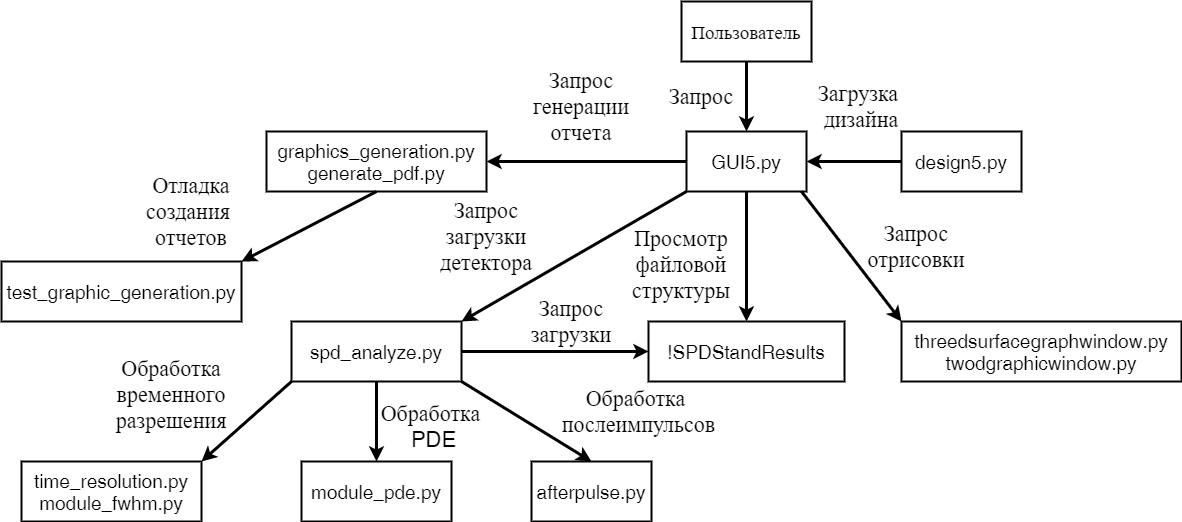
\includegraphics[width=1\textwidth]{program_scheme}
   \caption{Принципиальная схема работы программы обработки данных.}
   \label{fig:program_scheme}
\end{figure}



На рисунке \ref{fig:program_example2} представлен пример работы программы для обработки данных. Запуск возможен двойным нажатием на файл \verb|"start_SPD.bat"| или путем запуска скрипта в файле \verb|"GUI5.py"|. На данном рисунке красными прямоугольниками и нумерацией обозначены объекты, функции которых будут описаны ниже. 


\begin{figure}[h]\centering
	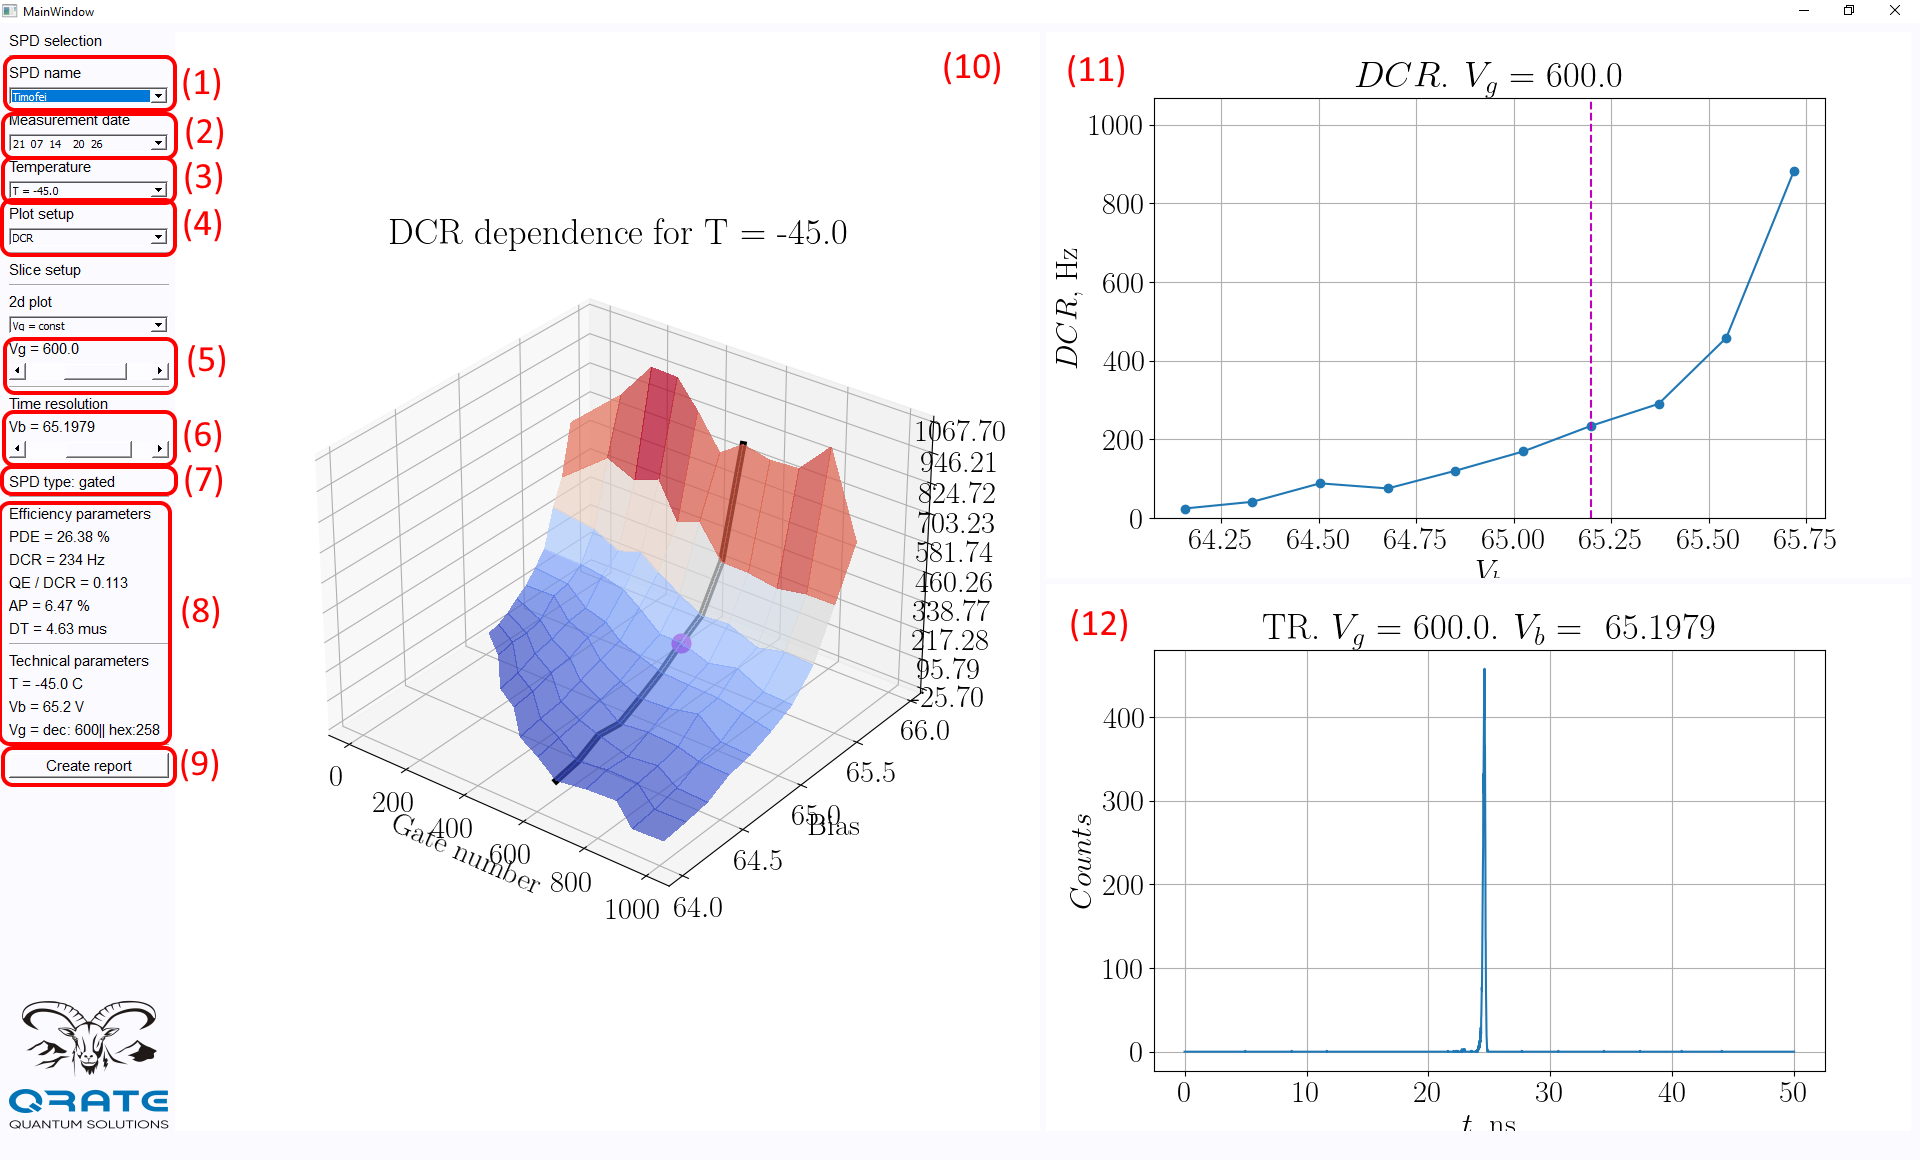
\includegraphics[width=1\textwidth]{program_example2}
   \caption{Пример окна приложения для обработки данных.}
   \label{fig:program_example2}
\end{figure}


Функции программы для обработки данных:

\begin{enumerate}
   \item SPD name. Выбор модели детектора. Каждый детектор носит свое имя, а не просто номер. На примере детектора "Тимофей".
   \item Measurement date. Выбор даты измерения детектора. Измерения, проведенные в разное время, могут иметь разные результаты. 
   \item Temperature. Выбор температуры, для которых будут отображаться все графики.
   \item Plot setup. Выбор  отображаемой характеристики на  графиках в 3-Д окне  (10) и в 2-Д окне (11).
   \item $V_g$. Выбор среза по коду строба -- выбор кода строба. Показан черной кривой на 3-Д графике. Именно при данной величине кода строба строится 2-Д график в окне (11).
   \item $V_b$. Выбор точки в срезе по коду строба -- напряжения смещения. Показан фиолетовой точкой на 3-Д графике и фиолетовой вертикальной пунктирной линией  на 2-Д графике. Характеристики детектора в данной точке представлены в окне (8).
   \item SPD type. Показывает тип исследуемого детектора. Либо freerun (фриран), либо gated (стробируемый).
   \item Efficiency and Technical parameters. Данные параметры определяются в указанной фиолетовым точке на 3-Д графике.  Параметры эффективности имеют эксплуатационную значимость для последующей интеграции устройство в систему квантового распределения ключа (КРК). Технические параметры нужны для настройки режима работы детектора. 
   \item Create report. Нажатие на кнопку формирует отчет по выбранной модели детектора и дате его измерения. Файл отчета сохраняется в папку \verb|report| в корне папки с данными детектора. 
   \item Окно 3-Д графика. На нем выводится тип графика, указанный в поле (4).
   \item Окно 2-Д графика. На нем выводится тип графика, указанный в поле (4), соответствующий срезу в поле (5).
   \item Окно 2-Д графика. На нем выводится график временного разрешения в точке, соответствующий фиолетовой точке на 3-Д графике.
\end{enumerate}

Для ДОФ типа фриран 3-Д график отсутствует в связи с отсутствием кода строба как варьируемого параметра. Таким образом, можно изменять только напряжение смещения в окне (6).




\begin{thebibliography}{}
   \bibitem{git} Ссылка на гитхаб с проектом: \verb|https://github.com/akoziy98/Automated_Stand|
   \bibitem{pyqt} Ссылка на ресурс по основам работы в PyQt: \verb|https://tproger.ru/translations/python-gui-pyqt/|
\end{thebibliography}


\end{document}





